\documentclass[a4paper, 12pt]{article}
\usepackage[total={17cm,25cm}, top=2.5cm, left=2.5cm, right=2.5cm,  includefoot]{geometry}
\usepackage[utf8]{inputenc}
\usepackage{array}
\usepackage{multirow}
\usepackage{hhline}
\usepackage{gensymb}
\usepackage{graphicx}
\graphicspath{ {} }
\usepackage[czech]{babel}
\usepackage{enumitem}
\usepackage{pdfpages}
\usepackage{amsmath}
\usepackage{verbatim}
\usepackage{listings}
\usepackage{hyperref}
\usepackage{amssymb}


\pagestyle{empty} % vypne číslování stránek




\usepackage[OT2,OT1]{fontenc}
\newcommand\cyr
{
\renewcommand\rmdefault{wncyr}
\renewcommand\sfdefault{wncyss}
\renewcommand\encodingdefault{OT2}
\normalfont
\selectfont
}
\DeclareTextFontCommand{\textcyr}{\cyr}
\def\cprime{\char"7E }
\def\cdprime{\char"7F }
\def\eoborotnoye{\char’013}
\def\Eoborotnoye{\char’003}
\setlength{\parindent}{1em} 
%\setlength{\parskip}{0.5ex}


\begin{document}

\begin{titlepage}
\begin{center}
%\noindent
\Huge
\vspace{4cm}
Algoritmy v digitální kartografii \\
\vspace{0.2cm}

\Large  
Geometrické vyhledávání bodu\\
\vspace{20cm}
\end{center}

\begin{flushright}
\Large
Tereza Kulovaná \\
Markéta Pecenová \\
\end{flushright}

\end{titlepage}


\pagestyle{plain}     % zapne obyčejné číslování
\setcounter{page}{1}  % nastaví čítač stránek znovu od jedné

\tableofcontents
\newpage

\section{Zadání}
\begin{figure}[h!]
	%\centering
	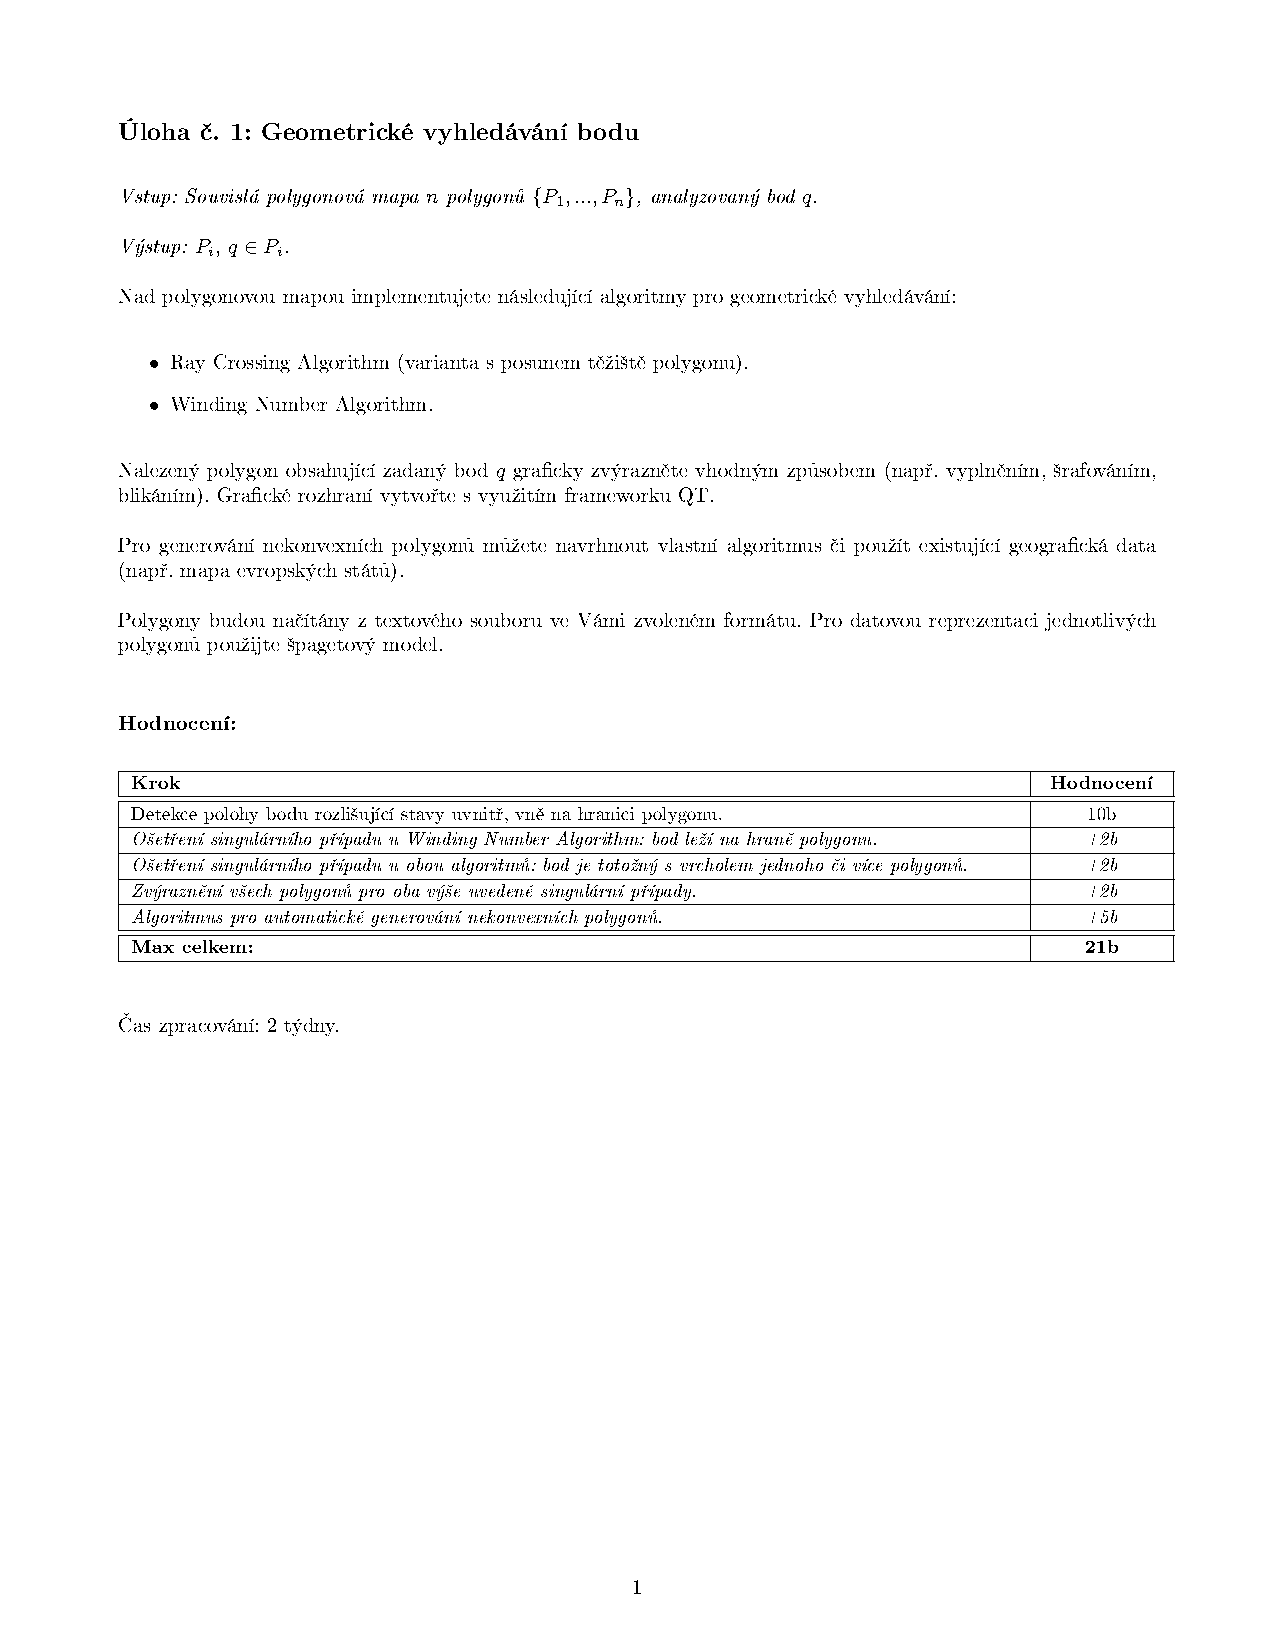
\includegraphics[clip, trim=0cm 10cm 0cm 3cm, width=1.0\textwidth]{./pictures/zadani.pdf}
\end{figure}

\subsection{Řešené bonusové úlohy}
\begin{enumerate}
\item 
%\item
%\item
\end{enumerate}


\clearpage

\section{Popis a rozbor problému}
Úloha \textit{Geometrické vyhledávání bodu} se zabývá vytvořením aplikace, která umožní uživateli zjistit polohu jím zvoleného bodu \textit{q} vzhledem k příslušnému mnohoúhelníku. Jako vhodné řešení bylo vzhledem k náročnosti problému zvoleno opakované určovnání polohy  bodu \textit{q} a mnohoúhelníku.

Existují dva základní druhy mnohoúhelníků (pro účely této úlohy je nazývejme polygony), konvexní a nekonvexní. Konvexní polygon je takový polygon, jehož všechny vnitřní úhly jsou menší nebo rovny 180$^\circ$. Konkávní polygon tuto podmínku nesplňuje. Pro představu je níže přiložen obrázek obou druhů polygonů.

\begin{figure}[h!]
	\centering
	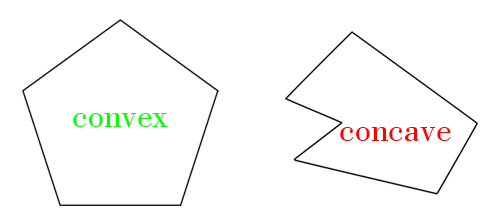
\includegraphics[width=13cm]{./pictures/convex_concave.png}
	\caption{Ukázka konvexního (vlevo) a konkávního polygonu (vpravo) (\href{https://www.nextgurukul.in/nganswers/ask-question/answer/What-is-concave-38-convex-polygon-/Understanding-Quadrilaterals/75323.htm}{\textsl{zdroj}})}
\end{figure}

Z výše uvedeného vyplývá, že bod \textit{q} může vůči polygonu \textit{P} nabývat 4 stavů:
\begin{enumerate}
\item Bod \textit{q} se nalézá uvnitř polygonu \textit{P}.
\item Bod \textit{q} se nalézá vně polygonu \textit{P}.
\item Bod \textit{q} se nalézá na hraně polygonu \textit{P}.
\item Bod \textit{q} se nalézá ve vrcholu polygonu \textit{P}.
\end{enumerate}

Pro účely této aplikace byly zvoleny výpočetní algoritmy \textit{Ray Crossing} a \textit{Winding Number}, jejichž princip je vysvětlen v následující kapitole.

\section{Algoritmy}
Tato kapitola se zabývá popisem algoritmů, které byly v aplikaci implementovány. 

\subsection{Ray Crossing Algorithm}
Prvním zvoleným algoritmem je tzv. \textit{Ray Crossing Algorithm} neboli \textit{Paprskový algoritmus}. Svůj název získal po metodě, jež využívá pro nalezení řešení polohy bodu vůči polygonu. Tento algoritmus je primárně využíván pro konvexní polygony, lze ho však zobecnit a využít ho i pro nekonvexní polygony. 

Mějme polygon \textit{P} a daný bod \textit{q}. Z bodu \textit{q} veďme libovolný počet polopřímek (paprsků). Princip algoritmu je založen na vyhodnocení počtu průsečíků \textit{k}, které vzniknou protnutím paprsků z vedených z bodu \textit{q} s hranami polygonu \textit{P}. Pro \textit{k} mohou nastat dvě situace:
\begin{enumerate}
\item Hodnota \textit{k} je rovna lichému číslu $\rightarrow$ bod q se nachází uvnitř polygonu  \textit{P}.
\item Hodnota \textit{k} je rovna sudému číslu $\rightarrow$ bod q se nachází vně polygonu \textit{P}.
\end{enumerate}

Základní varianta algoritmu neošetřuje problémové situace, které mohou během výpočtu nastat. Konkrétně se jedná o situace, kdy je bod q totožný s jedním z vrcholů polygonu P nebo pokud bod q leží na jedné z hran polygonu P. Pro eliminaci těchto tzv. singularit je vhodné použít modifikovanou variantu algoritmu, která redukuje souřadnice bodů polygonu k bodu q. 

Zjednodušený zápis takto modifikovaného algoritmu lze zapsat způsobem uvedeným níže:
\begin{enumerate}
\item Načtení bodů polygonu $p_i$, počet průsečíků $k$ = 0
\item Postupně pro všechny $p_i$ opakuj kroky 3-6
\item 	Redukce souřadnic bodu $p_i$ k bodu $q$:\\
$x'_i = x_i - x_q$\\
$y'_i = y_i - y_q$
\item 	Podmínka $(y'_i > 0)\&\&(y'_{i-1} <= 0)\|(y'_{i-1} > 0)\&\&(y'_{i} <= 0)$
\item 	Je-li podmínka splněna: $x'_m = \frac{x'_i y'_{i-1} - x'_{i-1} y'_i}{y'_i - y'_{i-1}}$
\item Splněno $(x'_m > 0) \rightarrow k = k + 1$ 
\item Výpočet $k\%2$
\item Vyhodnocení $k$ (liché $k$: $q$ náleží $P$, sudé $k$: $q$ nenáleží $P$)
\end{enumerate}

\subsection{Winding Number Algorithm}
Druhý algoritmus použitý v aplikaci je tzv. \textit{Winding Number Algorithm} neboli \textit{Metoda ovíjení}, který je vhodný pro nekonvexní polygony. Princip tohoto algoritmu je založen součtovém úhlu $\omega$.

Mějme polygon $P$ a bod $q$, na kterém stojí pozorovatel. Nachází-li se $q$ uvnitř $P$, pak pozorovatel, který by si přál postupně vidět všechny vrcholy polygonu, se musí otočit celkem o $2\pi$. Výsledkem algoritmu je pak tzv. Winding number $\omega$, které říká, o kolik otáček se pozorovatel otočil: \\ \\
$\Omega = \frac{1}{2\pi} \sum_{i=1}^n \omega_i^2$\\ \\
Zde se hodí zdůraznit, že záleží na zvoleném směru otáčení. Otáčí-li se pozorovatel ve směru chodu hodinových ručiček, uhly se sčítají. V opačném směru se odečítají a $\omega$ by vyšlo záporné. Během výpočtů je také nutno zavést určitou toleranci $\epsilon$, která pokrývá chyby způsobené zaokrouhlováním.
Z výše uvedených vztahů vyplývá:
\begin{enumerate} 
\item $w = 2\pi \rightarrow$ $q$ se nachází uvnitř $P$
\item  $w < 2\pi \rightarrow$ $q$ se nachází vně $P$
\end{enumerate}

Zjednodušený zápis algoritmu:

\begin{enumerate}
\item Načtení bodů polygonu, úhel $\omega = 0$, tolerance $\epsilon = 1e-10$
\item Postupně pro všechny orientované trojice $p_i, q, p_{i+1}$ opakuj kroky 3-5
%\item Určení orientace $o_i$ bodu q ke straně $p_i, p_{i+1}$
\item 	Výpočet úhlu $\omega_i = \sphericalangle p_i, q, p_{i+1}$
\item 	Podmínka (q je vlevo) $\rightarrow \omega = \omega + \omega_i$
\item 	Jinak $\omega = \omega - \omega_i$
\item Podmínka $(\omega - 2\pi) < \epsilon \rightarrow q \in P$
\item Jinak  $ q { \not \in } P $
\end{enumerate}
\section{Vstupní data}


\section{Výstupní data}

\section{Aplikace}

\section{Dokumentace}

\clearpage
\section{Závěr}

\clearpage
\section{Literatura}
\begin{enumerate}
\item  Presentation about convex and concave polygons [online][cit. 21.10.2018]. \\
Dostupné z: https://slideplayer.com/slide/6161031/  \\
\item  Introducing Wherewolf - A serverless boundary service from WNYC [online][cit. 21.10.2018]. \\
Dostupné z: https://source.opennews.org/articles/introducing-wherewolf/  \\
\item  BAYER, Tomáš. Geometrické vyhledávání [online][cit. 21.10.2018]. \\
Dostupné z: https://web.natur.cuni.cz/~bayertom/images/courses/Adk/adk3.pdf  \\

\end{enumerate}
\end{document}



 